\documentclass[]{auvsi_doc}
\setkeys{auvsi_doc.cls}{
	AUVSITitle={Wing Extensions Design Decision},
	AUVSILogoPath={./../logo.pdf}
}

% include extra packages, if needed

\begin{document}

\begin{AUVSITitlePage}
\begin{artifacttable}
\entry{AF-012, 0.1, 02-20-2019, Initial draft, Ryan Anderson, Tyler Critchfield}
% additional \entry{} commands for extra rows in the revision table, if needed
\end{artifacttable}
\end{AUVSITitlePage}

% document contents (see below for LaTex commands that make your life easier)
\section{Introduction}
In order to enhance the performance of our airframe, the XFLR5 model described in artifact AF-011 was extended to test the viability of wing extensions to further decrease the design speed of the airframe. As discussed in AF-011, a slower design speed will facilitate payload drop, waypoint navigation, and image capture- three of our key success measures. After this study, it was determined that wing extensions did not provide sufficient improvement to aerodynamic performance to warrant implementation.

\section{Method}
The decision not to implement wing extensions was reached by careful consideration of manufacturability and aerodynamic benefits, as follows.

\subsection{Manufacturability}
First, methods of adding wing extensions to the airframe were brainstormed. Each wing attaches to the fuselage by fitting two circular spars into two larger spars in the fuselage. A spring-loaded clipping mechanism is fitted to the root of each wing, and clips into the fuselage (see Fig. \ref{airfoil}). It was determined that up to 5~cm of foam section could be cut out of foam and fitted onto the spars on the root side of the wings. The clipping mechanism would be removed and replaced on the outside of the added foam section. Any more than 5~cm of extensions would require extensions on the spars. 

\begin{center}
	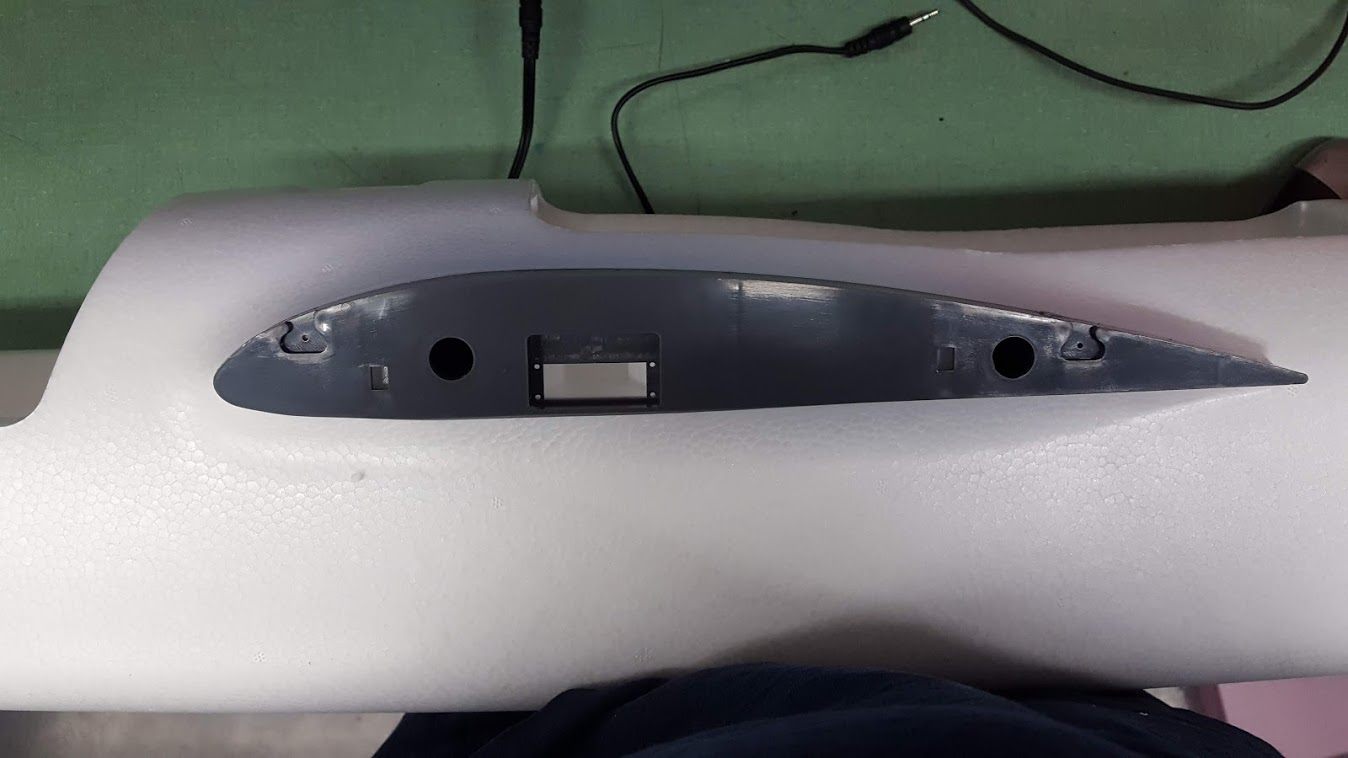
\includegraphics[width=0.95\textwidth]{./airfoils.png}
	\captionof{figure}{Clipping mechanism and spars for mounting wings. Fuselage is shown in this image.}
	\label{airfoil}
\end{center}

\subsection{Analysis}

In order to determine the aerodynamic advantage of wing extensions, the wings in the XFLR5 model were lengthened and an analysis similar to that described in AF-011 performed to predict the resulting design velocity.

\section{Results}

The model results are tabulated in Table \ref{data}. Note that only a very small decrease in speed is awarded by significant extensions of the wings. Note also that the design speed without any wing extensions is already significantly slower than last year's design. As a result, we decided not to add wing extensions.

\begin{table}[H]
	\centering
	\caption{Effect of wing extensions on design speed.}
	\label{data}
	\begin{tabular}{|P{3cm}|P{4.0cm}|}
		\hline
		\rowcolor[HTML]{C0C0C0}
		{\color[HTML]{000000} \textbf{Extension per Wing (cm)}} & {\color[HTML]{000000}\textbf{Design Speed (m/s)}} \\
		\hline
		0 & 12.863 \\
		\hline
		5.0 & 12.675\\
		\hline
		7.5 & 12.565 \\
		\hline
		10.0 & 12.459 \\
		\hline
	\end{tabular}
\end{table}

\section{Conclusion}

In summary, the aerodynamic performance of the aircraft was insufficiently enhanced by wing extensions to make them worth our while. We will devote time and other resources to other aspects of the project.


\end{document}
